\section{SVN/Subversion}
\subsection{Definition und Geschichte des SVN}
Der Begriff Subversion bzw. Subversion ist klar definiert. Der Begriff bezieht sich zum einen auf die politisch-soziologische Deutung der Subversion, die eine T�tigkeit im Verborgenen, deren Ziel der Umsturz einer bestehenden Ordnung durch Unterwanderung und Untergrabung ist, definiert. Desweiteren bezieht sich der Begriff auf die sub version, also Unterversion oder der fr�heren Version. Das bedeutet Subversion dient der Versionskontrolle. Mit SVN k�nnen verschiedene Entwickler an Dateien arbeiten. Dabei wird immer die aktuellste Version bereitgestellt, sodass alle Entwickler auf dem gleichen Stand sind. \\
Subversion wurde seit Anfang 2000 bei CollabNet entwickelt und erreichte Februar 2004 seine stabile Version 1.0. Seitdem wurden immer neuere Versionen entwickelt, die letzte ist die Version 1.5 (Juni 2008).Folgend werden die �nderungen in den einzelnen Versionen aufgelistet:
\begin{description}
 \item[Version 1.1] Repositories m�ssen nicht mehr in einer Berkley-Datenbank verwaltet werden, sondern man kann auch direkt das Dateisystem benutzen
 \item[Version 1.2] Die Sperrung von Dateien wurde eingef�hrt, was vor allem f�r bin�re Dateien hilfreich ist
 \item[Version 1.3] Das Server-Logging, die Autorisierung, die Programmiersprachen-Anbindung, die Kommando-Option und die Leistung wurden verbessert
 \item[Version 1.4] svnsync bietet das Spiegeln von Projektarchiven an
 \item[Version 1.5] Merge-Tracking und das sparse checkout wurden eingef�hrt
\end{description}
\newpage
\subsection{Arbeitsweise des SVN und Vorteile}
SVN arbeitet eigentlich wie das immer noch weitverbreitete CVS, welches viele Schw�chen aufweist. SVN bietet eine Versionsverwaltung im Sinne einer einfachen Revisionsz�hlung. Dabei werden die zu bearbeitenden Daten in einem Repository abgelegt. Falls �nderungen an den Dateien vorgenommen werden, werden lediglich die Unterschiede zwischen dem Repository und dem lokalen System �bertragen. 
\begin{center}
\begin{figure}[!h]
 \fbox{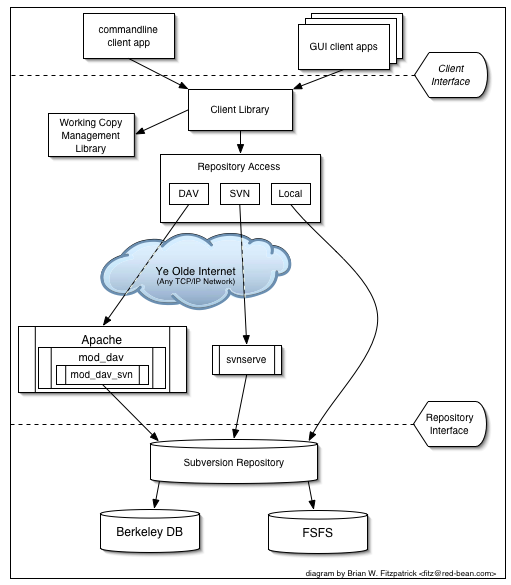
\includegraphics[scale=0.5]{subversion-diagram.png}}
 \caption{Subversion-Diagramm}
 \label{Subversion-Diagramm}	
\end{figure}
\end{center}
Das Diagramm erl�utert die Vorgehensweise des SVN in allen drei Schichten (User-Schicht, SVN-Schicht und Repository-Schicht). �ber eine Applikation oder �ber die Kommandozeile gibt der User seine Interaktion an. Daraufhin greift SVN mittels des Befehls auf das Repository zu (�ber DAV, SVN oder lokal) und f�hrt den Befehl auf dem Repository aus. Je nach Befehl werden Dateien hochgeladen, runtergeladen, hinzugef�gt, gel�scht, gemerged etc.\\
SVN bietet zwei unterschiedliche Backends zur Verwaltung der Repositorys an. Das eine ist die \emph{Berkley-Datenbank} und das andere ist das \emph{fsfs-Backend}. In der folgenden Tabelle werden die Unterschiede und Gemeinsamkeiten aufgelistet:
\begin{center}
% use packages: array
\begin{tabular}[c]{|p{6cm}|p{6cm}|}
\hline
Berkley-Datenbank & fsfs-Backend \\ \hline 
Speichert das Repository in einer Datenbank & Speichert das Repository in einer einzigen Datei \\ \hline
Transaktionen werden in der Datenbank gespeichert & Transaktionen werden als Unterordner gespeichert \\ \hline
Die Gr��e und der Zugriff spielen keine Rolle & Die Gr��e ist kleiner und der Zugriff ist nicht unbegrenzt \\ \hline
Benutzt einen $O(n�)$-Algorithmus, um den kompletten Ordner zu �berschreiben & Benutzt einen O(n) -Algorithmus, um die Dateien an das Repository ranzuh�ngen \\ \hline
Auscheken des letzten Baumes ist schnell & Auschecken des letzten Baumes ist etwas langsamer \\ \hline
Beim Crash bleibt die DB unbrauchbar bis sie repariert wird & Beim Crash ist nicht das komplette Repository betroffen, sondern evtl. nur die Transaktion \\ \hline
Repository-Backup funktioniert zur Laufzeit & Repository-Backup funktioniert zur Laufzeit \\ \hline
Repository kann nicht auf andere OS kopiert werden & Repository kann auf andere OS portiert werden\\ \hline
\end{tabular}
\end{center}
\vspace{1cm} 

Im Gegensatz zu CVS bietet SVN einige Merkmale, die das Arbeiten sehr viel einfacher gestalten. In der folgenden Liste, sind die Vorteile gegen�ber CVS aufgelistet:
\begin{itemize}
 \item SVN versioniert oder revisioniert grunds�tzlich das gesamte Projektarchiv und damit jeweils die gesamte Verzeichnisstruktur, w�hrend CVS auf der unabh�ngigen Versionierung jedes einzelnen Inhalts beruht
 \item  Mit Subversion ist es m�glich, Dateien oder Verzeichnisse zu verschieben oder umzubenennen, ohne die Versionsgeschichte zu verlieren
 \item �nderungen ("commits") sind  in Subversion atomar, das hei�t, eine �nderung wird entweder ganz oder gar nicht ins Repository gespeichert. Verbindungsabbr�che und mehrere gleichzeitige "commits" k�nnen somit nicht zu inkonsistenten Zust�nden f�hren
\end{itemize}
